\documentclass[parskip=full]{scrartcl}

\pdfoutput=1

\title{G-SOMO \\ \LARGE{An Oversampling Approach based on Self-Organized Maps and Geometric SMOTE}}

\author{
	Georgios Douzas\(^{1}\), Fernando Bacao\(^{1*}\), Rene Rauch\(^{1}\)
	\\
	\small{\(^{1}\)NOVA Information Management School, Universidade Nova de Lisboa}
	\\
	\small{*Corresponding Author: bacao@novaims.unl.pt}
	\\
	\\
	\small{Postal Address: NOVA Information Management School, Campus de Campolide, 1070-312 Lisboa, Portugal}
	\\
	\small{Telephone: +351 21 382 8610}
}

\usepackage{breakcites}
\usepackage{float}
\usepackage{graphicx}
\usepackage{geometry}
\geometry{
	a4paper,
	total={170mm,257mm},
	left=18mm,
	right=18mm,
	top=8mm,
}
\usepackage{amsmath}
\newcommand{\inlineeqnum}{\refstepcounter{equation}~~\mbox{(\theequation)}}
\usepackage{enumitem}
\usepackage[ruled,vlined]{algorithm2e}
\usepackage{booktabs}
\usepackage{pgfplotstable}
\usepackage{longtable}
\usepackage{tabu}
\usepackage{hyperref}
\date{}

\begin{document}

\maketitle

\begin{abstract}
Traditional supervised machine learning classifiers are challenged to learn
highly skewed data distributions as they are designed to expect classes to
equally contribute to the minimization of the classifiers cost function.
Moreover, the classifiers design expects equal misclassification costs, causing
a bias for underrepresented classes. Thus, different strategies to handle the
issue are proposed by researchers. The modification of the data set has become a
common practice since the procedure is generalizable to all classifiers. Various
algorithms to rebalance the data distribution through the creation of synthetic
instances were proposed in the past.  In this paper, we propose a new
oversampling algorithm named G-SOMO, a method that is adopted from our previous
research. The algorithm identifies optimal areas to create artificial data
instances in an informed manner and utilizes a geometric region during the data
generation to increase variability and to avoid correlation. Our empirical
results on 69 datasets, validated with different classifiers and metrics against
a benchmark of commonly used oversampling methods show that G-SOMO consistently
outperforms competing oversampling methods. The statistical significance of our
results is proven. 
\end{abstract}

\section{Introduction}

Learning from imbalanced datasets is a pervasive and challenging problem in
supervised machine learning. Imbalanced datasets are common in many application
domains such as are fraud detection, medical diagnosis, risk management,
airborne imagery, face recognition and forecasting of ozone levels and can be
seen as a form of data scarcity \cite{Vong2014}, \cite{He2009}. The recent
growth in the number of research papers on the topic \cite{Haixiang2017},
\cite{Fernandez2018},  suggests that it continues to be a relevant and important
topic for the research community.

The imbalanced learning problem can be defined as a classification problem where
there is a substantial asymmetry between the number of instances of the classes.
The dominant class is called the majority class while the other classes are
called the minority classes \cite{Chawla2003}. The Imbalance Ratio (IR) is the
measure commonly used to assess the imbalance severity in datasets. The IR is
defined as the ratio between the majority class and the minority class, and it’s
frequent to find values between 100 and 100.000 \cite{Chawla2002},
\cite{Barua2014}.

Imbalanced datasets constitute a problem insofar as standard machine learning
methods induce a bias in favor of the majority class during training. This
happens because the minority classes contributes less to the minimization of
accuracy, the commonly used objective function. It is well known that accuracy
is heavily biased towards the majority class, and can be misleading when
assessing the performance of a classifier. For instance, assuming a dataset with
\( 99\% \) majority instances and only \( 1\% \) minority instances, the model
accuracy would still be \( 99\% \) without classifying a single minority
instance correctly.

It is also important to note that most methods assume equal costs in the
misclassification of minority and majority instances, but this is seldom the
case. Very often, the misclassification costs associated with the
misclassification of minority instances (false negatives) is much higher than
the misclassification of majority instances (false positives)
\cite{Domingos1999}, \cite{Ting2002}. Diseases screening tests are just an
example of the situation in which false negatives involve a much higher cost
than the false positives \cite{Wan2014}.

In general, there are three different options to handle an imbalanced datasets
\cite{Fernandez2013}. One is to adjust the cost function of the algorithm, which
means that during the training process, the model will be heavily penalized for
misclassifying minority instances (false negatives). This can be a laborious
process as it involves the modification of the training process for every
algorithm the user applies. Another option is to focuses on the modification of
algorithms reinforcing the learning towards the minority class. Again, this can
be a complex and lengthy procedure, possibly restricting the algorithm options
available to the user. Finally, the last option is to modify the data. This can
be done by generating new synthetic data instances of the minority classes,
known as oversampling, or by removing instances from the majority class, known
as undersampling. The objective of both, oversampling and undersampling, is to
balance the dataset, minimizing the skewness of the data distribution.

In this paper we adopt this last option, and tackle imbalanced learning problem
by re-balancing class distribution through oversampling. This is a more general
approach, because once the distribution is balanced any supervised machine
learning algorithm can be used, without any further modification. Additionally,
by using oversampling, and contrary to undersampling, no data is wasted, as none
of the majority instances need to be removed.

The oversampling process can be divided into two steps: a) the process of
choosing where to generate the synthetic minority instances; b) the actual
process of generating the synthetic minority instances. Both of these processes
are essential for a successful oversampling process. These two steps should
prevent the generation of synthetic minority instances in areas of the input
space dominated by majority instances.

The method presented in this paper extends the Self-Organizing Map Oversampling
algorithm (SOMO) \cite{Douzas2017}, shown to be particularly efficient in
identifying areas where the synthetic minority instances should be generated, by
coupling it with the Geometric SMOTE algorithm (G-SMOTE) \cite{Douzas2019}, used
as the generation process of the minority instances.

SOMO is a clustering based oversampling algorithm based on the Self-Organizing
Map (SOM) algorithm and as been shown to outperform related algorithms over
various datasets. The algorithm preserves the topology of the input space, while
reducing the dimensionality to a two-dimensional representation. The emerging
clusters are then used as a map to guide the generation of minority instances
within, but also between neighboring minority clusters. In the original SOMO
paper the generation process was done through the application of the SMOTE
algorithm.

The new algorithm presented in this paper (G-SOMO) uses SOMO to identify the
areas to populate with synthetic minority instances, but replaces SMOTE with
G-SMOTE as the data generation mechanism. G-SMOTE generates synthetic samples in
a geometric region of the input space, around each selected minority instance.
It has been shown that G-SMOTE produces significant improvements in the
generated data quality. We evaluate G-SOMO performance using 69 datasets, 4
different classifiers and 3 different performance measures and compare it with
random oversampling and SMOTE.

In the next section we will outline related methods that proved to be efficient.
In section 3, we explain some of the shortcomings of classifiers and other
oversampling methods and explain the motivation for using G-SOMO. Next, we
explain in detail the G-SOMO algorithm, followed by a presentation of
experimental setup used to produce the results and validate the performance of
the different methods. In section 6 the results and their statistical analysis
are presented. The last section summarizes our findings and provides some ideas
for further research.

\section{Related work}

The section outlines the current state of the art oversampling methods.
Oversampling methods generate synthetic examples for the minority class and add
them to the training set, therefore additional information is created. In
contrast to oversampling, undersampling methods reduce samples of the majority
class to establish a class balance This implies that information is excluded,
which might affect the learning process negatively, especially when the data set
is small. Both methods have shown to be effective, depending on the problem
addressed \cite{Chawla2002}. More information on undersampling methods can be
found in \cite{Ganganwar2012} and \cite{Yen2006}. Synthetic data instances can
be created uninformed, by randomly duplicating minority instances or informed,
by identifying areas where oversampling is deemed to be most effective
\cite{Douzas2018}.

The simplest form of oversampling is Random Oversampling (ROS). ROS is an
uninformed approach, which randomly selects minority samples and duplicates them
exactly without any selection criteria. The method stands out through its
simplicity, but significantly increases the risk of overfitting, since the same
information is used multiple times during the training process, no instances
that clarify the decision boundaries are created. 

The most popular approach among practitioners in the domain of oversampling is
SMOTE, introduced in 2002. The algorithm chooses a random minority instance and
identifies its \( k \) nearest neighboring minority instances. The parameter \(k
\) is chosen beforehand. A synthetic instance is created on a random point along
the line segment joining the selected minority instance and one of its neighbors
\cite{Chawla2002}.  Depending upon the amount of oversampling required,
neighbors from the \( k \) nearest neighbors are randomly chosen. Figure
\ref{fig:Schubach} constitutes the process of SMOTE.

\begin{figure}[H]
	\centering
	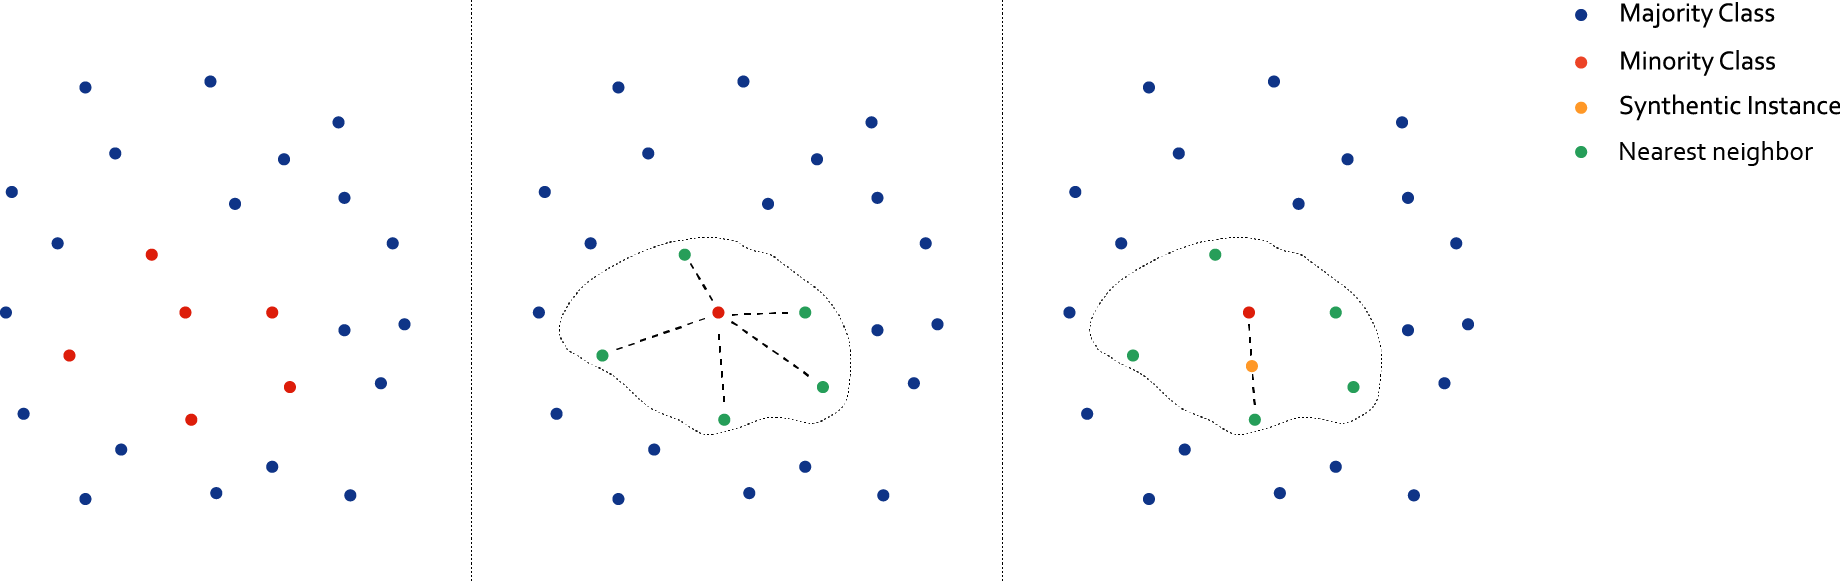
\includegraphics[width=16.5cm, height=5cm, keepaspectratio]{./resources/fig1.png}
	\captionbelow{SMOTE Algorithm, adopted from \cite{Schubach2017}}
	\label{fig:Schubach}
\end{figure}

Compared to ROS, the synthetic samples are more generalizable and therefore the
high risk of overfitting is reduced. However, SMOTE has several drawbacks.
First, the algorithm randomly selects a minority instance for oversampling with
uniform probability. Therefore it tackles between-class imbalance, while
within-class imbalance is ignored. Areas that were highly populated by minority
samples will expand, while smaller areas of minority samples will remain sparse
\cite{Prati2004}. Second, the algorithm promotes the generation of noisy
samples. When selecting a noisy sample and the linear interpolation to the
nearest neighbor is created, a new noisy sample might be created, due to the
great distance between them. It can not distinguish overlapping class regions
from safe areas \cite{Bunkhumpornpat2009}. 

To tackle the problems of SMOTE several modifications were created. SMOTE +
Edited Nearest Neighbor removes any misclassified instances after the creation
of synthetic samples, by applying the edited nearest neighbor rule
\cite{Batista2004}. Safe-Level SMOTE applies a weight degree to differentiate
between noisy and safe instances \cite{Bunkhumpornpat2009}. Furthermore, G-SMOTE
manages to extend the linear interpolation of SMOTE by introducing a geometric
region where the data generation process occurs. Thereby, the algorithm
increases the data variability and prevents additional correlation between the
created samples \cite{Douzas2019}. Further algorithms like Borderline-SMOTE
\cite{Han2005}, MWMOTE (Majority Weighted Minority Oversampling Technique for
Imbalanced Data Set Learning) \cite{Barua2014}, ADASYN and its variation
KernelADASYN \cite{Tang2015} are trying to avoid noisy samples and focus on hard
to learn instances. Hereby, the borderline samples of the classes are identified
to use the informative minority class instances.

The prior algorithms focus exclusively on between-class imbalance
\cite{Nekooeimehr2016}. The second challenge is an informed approach, the
within-class-imbalance. Within-class-imbalance refers to identifying sparse or
dense clusters of minority or majority instances. To tackle this challenge,
different clustering based oversampling methods have been proposed to identify
areas, where oversampling is most effective. These methods are segmenting the
instances and then apply traditional oversampling methods specific to each
segment. 

Cluster SMOTE utilizes the k-means cluster algorithm, to identify clusters with
a specific threshold of minority instances, before applying SMOTE within these
clusters \cite{Cieslak2006}. In addition, K-means and SMOTE applies a similar
approach, but also considers the density within the clusters by assigning
samples weights. A high sampling weight corresponds to a low density of minority
samples and yields more generated samples \cite{Douzas2018}. Furthermore, multiple
suggestions for the hyper-parameter selection are provided. DBSMOTE provides
another approach to cluster based oversampling, by applying the density-based
DBSCAN algorithm to discover arbitrarily shaped clusters to create artificial
data instances along the shortest path from each minority class instance to a
pseudo-centroid of the cluster \cite{Bunkhumpornpat2012}. A-SUWO uses a
hierarchical clustering approach and adaptively determines the size to
oversample each sub-cluster using its classification complexity and
cross-validation \cite{Nekooeimehr2016}. 

The Self Organizing Map Oversampling (SOMO) algorithm applies a self-organizing
map to create a two-dimensional representation of the multidimensional input
space and creates inter-cluster and intra-cluster synthetic samples based on the
underlying manifold structure \cite{Douzas2017}. The algorithm transforms the
input in a two-dimensional space of clusters and applies the SMOTE oversampling
algorithm to generate synthetic instances in the minority clusters and between
neighboring minority clusters. The densities in and between the clusters are
also taken into account by utilizing the average Euclidean distance. The
algorithm stands out through its ability to not only oversample the identified
clusters, but also between neighboring minority clusters since those areas are
also safe and effective for data generation.  

Besides clustering based algorithms, further oversampling algorithms have been
proposed, that are based on ensemble methods like SMOTEBoost \cite{Chawla2003}
and DataBoost-IM \cite{Guo2004}. The boosting process is used to identify hard
to learn instances, which are used to separately generate synthetic examples for
the majority and minority classes  \cite{Guo2004}.

\section{Motivation}

The section briefly outlines the challenges and shortcomings of competitive
oversampling methods and clarifies the motivation for our proposed algorithm
G-SOMO.

A classifiers performance is significantly influenced by the positioning of the
instances in the dataset. As outlined in figure \ref{fig:Sez}, the instances of
a class can be spread over the boundaries of the majority class, which
complicates the classifiers task \cite{Tang2007}. This is a common challenge in
real-world problems. The different types of instances can be seen as safe and
unsafe instances, while the latter also differentiate between borderline and
outlier instances \cite{Sez2016}.

\begin{figure}[H]
	\centering
	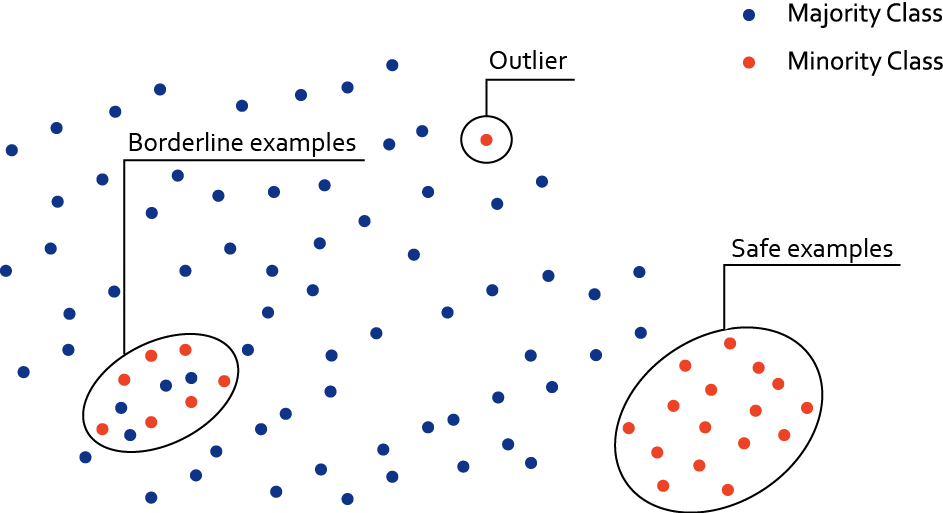
\includegraphics[width=10cm,height=7cm, keepaspectratio]{./resources/fig2.png}
	\captionbelow{Challenging data formations, adopted from  \cite{Sez2016}.}
	\label{fig:Sez}
\end{figure}

Safe instances are located in the homogeneous regions and populated by the
examples from one class only \cite{rodriguez2012}. They are clearly
separated from examples of other classes. Most classifiers are able to correctly
identify those instances \cite{Prati2004B}. Instances that are not clearly
separated are considered unsafe ones like borderline instances and outliers
\cite{Kubat1997}. Borderline instances are placed in the boundary region between
classes, where instances of multiple classes overlap \cite{Sez2016}. Outliers are
isolated distinct instances, also termed as noise. 

Learning algorithms are challenged when they are confronted with overlapping
areas between classes, especially unsafe instances. Therefore, oversampling
algorithms should be able to carefully consider in which areas to create
artificial instances and which areas to ignore. Inefficiencies that were
observed with SMOTE and similar algorithms are the generation of noisy instances
penetrating the area of majority classes, as well as the generation of nearly
duplicated examples. Noisy examples can be created when applying k-nearest
neighbor approaches, since they can either choose a noisy instance as a starting
point or select a noisy instance as nearest neighbor, as seen in figure 3a and
3b. Similar or nearly duplicated instances are created while generating new
artificial instances within the borders of a minority cluster since they do not
help to strengthen the decision boundary and might lead to overfitting, as it
can be seen in figure 3c. Figure 3d outlines the case, in which the parameter k
is too high and individuals from another cluster are selected.

\begin{figure}[H]
	\centering
	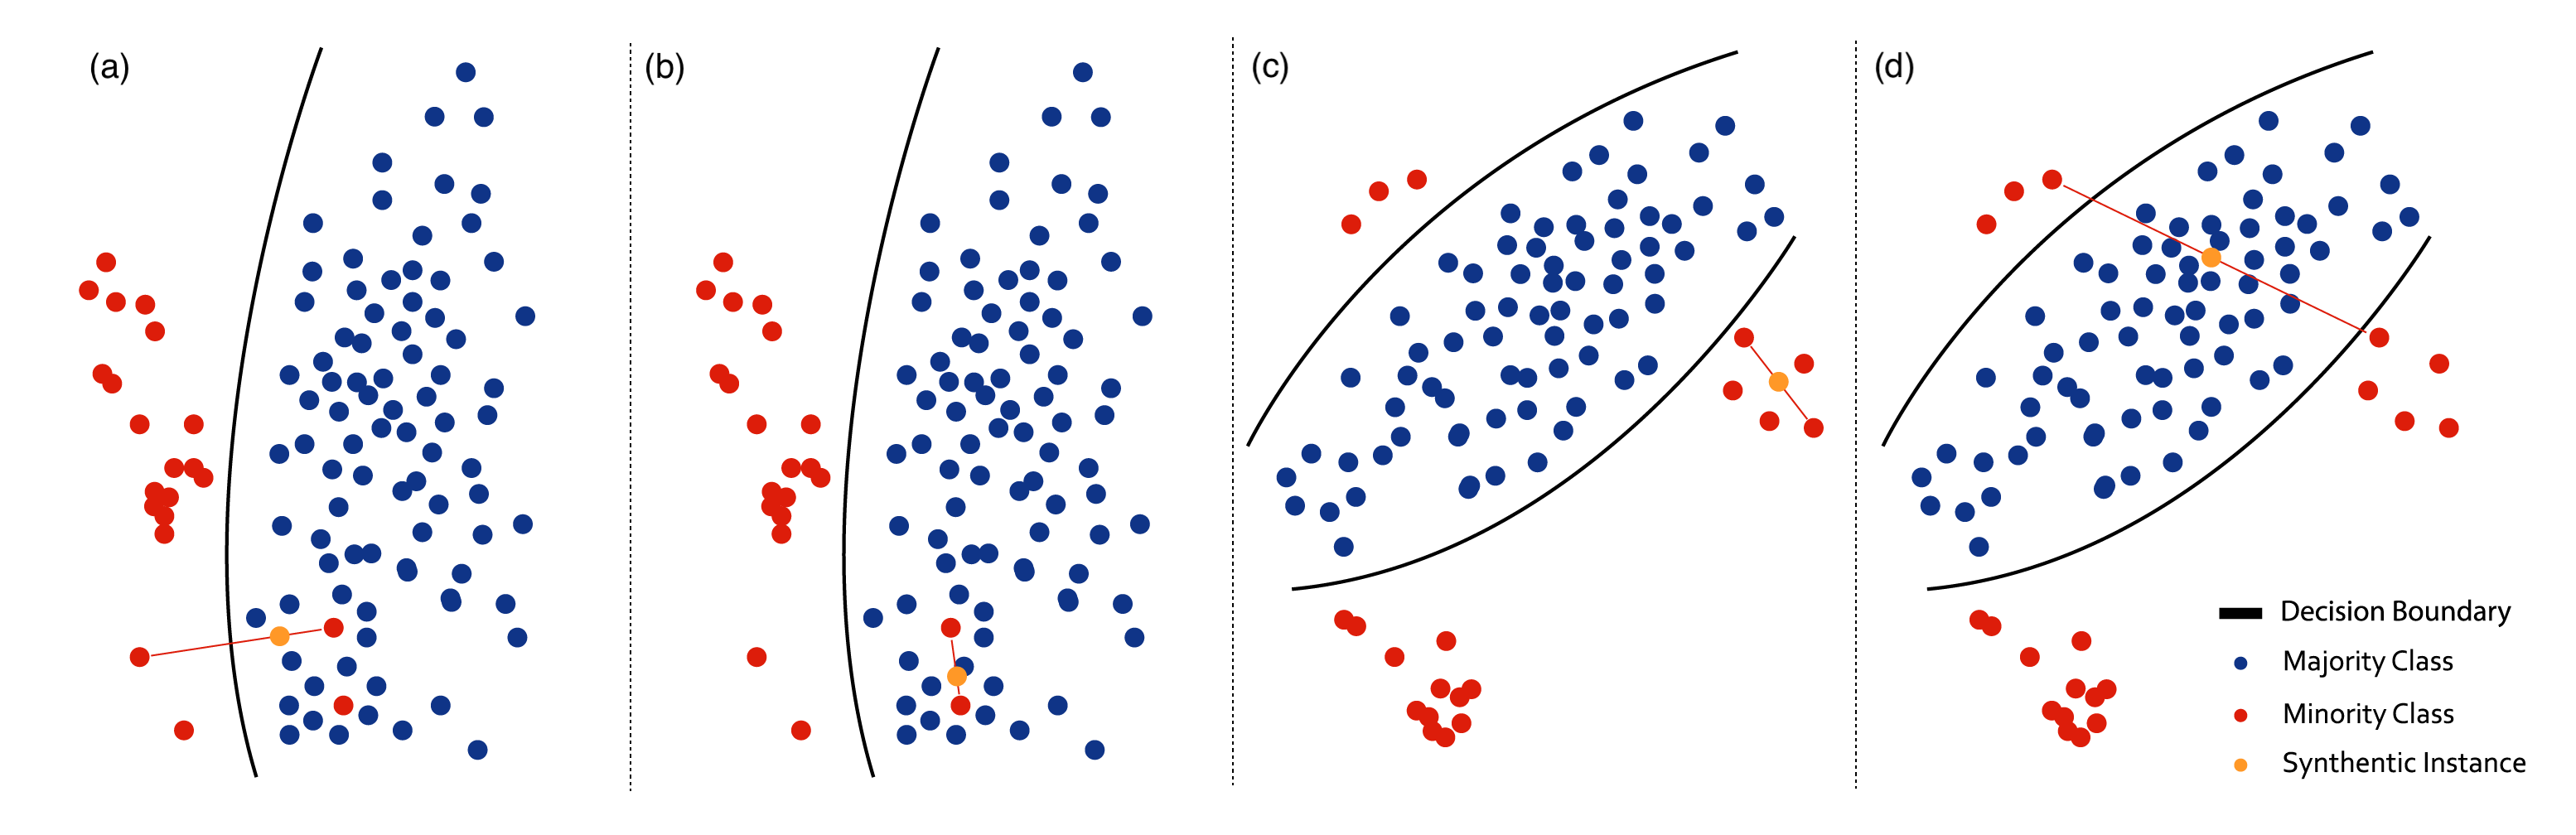
\includegraphics[width=16.5cm, height=14cm, keepaspectratio]{./resources/fig3.png}
	\captionbelow{Shortcomings of SMOTE, adopted from \cite{Douzas2017}}
\end{figure}

The Self-Organizing Map Oversampling (SOMO) algorithm improved the selection
criteria of the minority class samples, which are used to generate synthetic
examples. Through the synthetic data generation in and between neighboring
minority clusters, as well as the consideration of the density, the algorithm
also manages to generate the synthetic instances in more productive areas of the
data space \cite{Douzas2017}. Therefore, the generation of noisy examples is
avoided. SOMO manages to identify efficient oversampling areas, the generation
of synthetic instances is then handled by the SMOTE algorithm, which still
provides several drawbacks. Challenges, as outlined in figure 3d, are prevented
through the previous generation of clusters, nevertheless, the SMOTE algorithm
introduces a high correlation between the samples, since it only creates
synthetic instances that are on the line segment between two instances.

Geometric SMOTE (G-SMOTE) extends the linear interpolation mechanism by
introducing a geometric region, in which the data generation process occurs
\cite{Douzas2019}. Therefore, the algorithm extends the linear interpolation
mechanism and provides a geometric region in which the data generation occurs.
Figure \ref{fig:GSMOTE} illustrates the idea behind the data generation based on a geometric
region, instead of on the line segment. 

\begin{figure}[H]
	\centering
	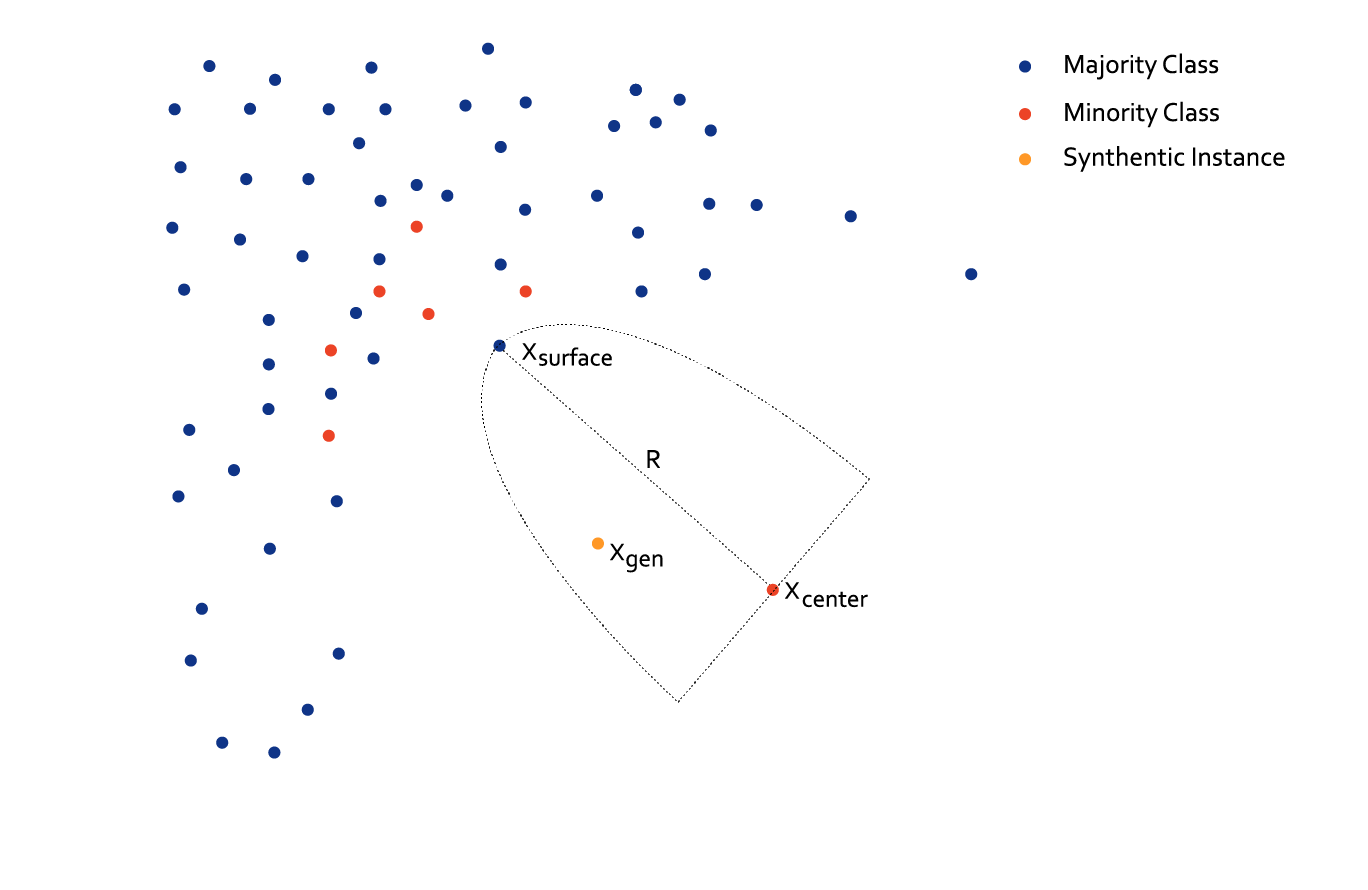
\includegraphics[width=12cm, height=9.5cm, keepaspectratio]{./resources/fig4.png}
	\captionbelow{Synthetic data generation based on a geometric region, adopted from \cite{Douzas2019}}
	\label{fig:GSMOTE}
\end{figure}

Besides utilizing a geometric region for the data generation, G-SMOTE also
introduced the majority selection strategy, which successfully prevents the
scenario shown in figure 3a, 3b and 3d. The majority selection strategy prevents
the creation of synthetic instances between two minority instances if the
distance to a majority instance is shorter. Instead, the synthetic minority
instance is created between the initially selected minority instance and the
majority instance that had a shorter distance, as it can be seen in figure \ref{fig:GSMOTE}.
G-SMOTE proved to significantly increase the performance of SMOTE. 

SOMO provides an efficient process to identify areas that should be populated
with minority instances, but lacks the improvements provided by G-SMOTE. On the
other hand, G-SMOTE exploits an intelligent and efficient approach to generate
synthetic instances, but lacks the ability to identify attractive regions for
synthetic instances. In this paper we propose a combination of both techniques,
leveraging the benefits of both algorithms. 

\section{Proposed method}

The previous section outlined the inefficiencies of the SMOTE algorithm, as well
as of SOMO and G-SMOTE. The proposed method, G-SMOTE, manages to tackle them, by
utilizing the best characteristics of both algorithms: It improves the selection
criteria by leveraging Self-Organizing Maps. The method considers the density,
based on the average Euclidean distances, in and between clusters when creating
artificial data instances. Also, G-SOMO creates synthetic instances within a
geometric region, avoiding correlation between the instances. Finally, through
the combined selection strategy, the creation of noisy examples is avoided. This
should already be prevented through the preselection of minority clusters, but
still provides an advantage, in case the parameters to cluster were not selected
carefully.

The proposed method consists of three stages:

\begin{enumerate}

	\item Initially, a Self-Organizing Map (SOM) is applied to the normalized
		  input data set. The SOM algorithm creates a mapping of the high
		  dimensional data space into a low-dimensional space in such a way that
		  the topological relations of the input patterns are preserved
		  \cite{Kker2007}. To train a SOM, the Euclidean distance between the
		  input vector and all neural weights has to be calculated. The neuron
		  that has the shortest distance to the input vector (the winner) is
		  chosen and its weights are slightly modified to the direction
		  represented by the input vector. Afterward, the neighboring neurons
		  are taken and their weights are modified in the same direction
		  \cite{Brocki2007}. Due to SOMs ability to preserve topological
		  relations from high dimensional input spaces, insights in the
		  underlying data structure can be retrieved by analyzing the (usually)
		  two-dimensional output map. 
	
	\item In the second stage of the algorithm, the filtered clusters are
		  defined, i.e. clusters where the minority class is dominating over the
		  majority class. A weighted approach is used to create synthetic
		  instances in the filtered clusters and also between neighboring
		  filtered clusters. 
		  
	\item The last stage of the algorithm is marked by the creation of synthetic
		  instances within the identified formations. The synthetic data
		  generation is based on a geometric region, that is formed between the
		  current minority instance and its selected neighbor. The shape of the
		  geometric region varies, depending on its hyper-parameter. Synthetic
		  instances are created within the geometric region, avoiding the
		  creation on a line segment as suggested by SMOTE.

\end{enumerate}

\subsection{G-SOMO Algorithm}

The G-SOMO algorithm is the efficient combination of the SOMO and G-SMOTE
algorithm, introduced in \cite{Douzas2017} and \cite{Douzas2019}. The complete
G-SOMO algorithm is listed below:

\begin{algorithm}[H]

	\SetAlgoLined
	\caption{Pseudo code for G-SOMO implementation}
	
	\BlankLine
	
	\SetKwInOut{Input}{Input}
	\SetKwInOut{Output}{Output}
	
	\Input{$S_{maj}$, $S_{min}$, $N_{intra}$, $N_{inter}$, $IR_{f}$, $SOM_{parameters}$, $\alpha_{trunc}$, $\alpha_{def}$, $\alpha_{sel}$}

	\BlankLine

	\textbf{Algorithm}
	\SetAlgoLined

	\begin{enumerate}

		\item Train a SOM with $SOM_{parameters}$ on the input data set. Define
			  as $cl$ the collection of randomly assigned cluster labels on the
			  SOM nodes that contain at least one minority class instance.
	
		\item Define $cl_{f} =\{i \in cl: IR^{i} < IR_{f} \} $ and 	
			  $cl_{f, n} =\{(i, j) \in cl_{f} \times cl_{f}: i, j \text{ topological neighbors } \} $ 
			  where $IR^{i}$ is the $IR$ of  $i$ cluster.
	
		\item Calculate the density factor for each $i \in cl_{f}$  as $den^{i}
			  = \dfrac{n^{i}_{+}}{(dist^{i})^2}$ and for each $(i, j) \in cl_{f, n}$ 
			  as $den^{i, j} = den^{i} + den^{j}$ where $n^{i}_{+}$ is the
			  number of minority class samples in $i$ cluster and $dist^{i}$ is
			  the sum of Euclidean distances between all pairs  of minority
			  class samples in $i$ cluster.
	
		\item Calculate the sampling weights for the intra-cluster case as
			  $w^{i}_{intra} = \dfrac{1 / den^{i}}{\sum_{i \in cl_{f}} 1/den^{i}}$ and
			  for the inter-cluster case as 
			  $w^{(i, j)}_{inter} = \dfrac{1 / den^{(i, j)}}{\sum_{i,j \in cl_{f}} 1/den^{(i,j)}}$.
	
		\item Calculate the number of artificial instances to be created for
			  each $i \in cl_{f}$ from $[w^{i}_{intra} \cdot N_{intra}]$ and for
			  each $(i, j) \in cl_{f, n}$ from $[w^{(i, j)}_{inter} \cdot N_{inter}]$.

		\item Define as $S_{min, i}$ and $S_{maj, i}$ the sets of minority and
			  majority class instances for $i$ cluster, respectively. 
			  Set $S_{synthetic} = \emptyset$.
	
		\item For each $i \in cl_{f}$ and each $(i, j) \in cl_{f, n}$ repeat the following:
		
			\begin{enumerate}[label*=\arabic*.]
		
			\item Shuffle $S_{min, i}$. 
		
			\item Repeat until the calculated number of instances from step 6 is created:
				  
				\begin{enumerate}[label*=\arabic*.]

				\item Select $x_{center}$ from $S_{min, i}$.
				
				\item Apply the $\alpha_{sel}$ selection strategy and calculate
					  a radius $R$. For the case of neighboring filtered
					  clusters, use $S_{min, j}$ and $S_{maj, j}$ to search for
					  the nearest neighbors.
				
				\item Generate a random point inside the unit-hypersphere
					  centered at the origin of the input space.
				
				\item Truncate the unit hyper sphere using $\alpha_{trunc}$
					  hyper-parameter.
				
				\item Deform the unit hyper sphere to a hyper spheroid using
					  $\alpha_{def}$ hyper-parameter.
				
				\item Rescale the created sample $x_{gen}$ using the radius $R$.
				
				\item Add the sample $x_{gen}$ to the set $S_{synthetic}$ of
					  generated instances.

				\end{enumerate}

			\end{enumerate}

	\end{enumerate}

	\Output{ $S' = S_{maj} \cup S_{min} \cup S_{synthetic}$} 	

\end{algorithm}

\subsection{Explanation of G-SOMO}

The G-SOMO algorithm relies on filtered clusters, which are areas where a
specific minority class dominates over the majority class. These regions can be
considered as safe areas for the generation of minority samples. Outliers or
noisy examples should belong to non-filtered clusters and are therefore ignored.
The density and weights of each filtered cluster are calculated to create new
instances in each filtered cluster (intra-luster) and between filtered clusters
that are neighbors on the topological output map of the SOM algorithm
(inter-cluster). The geometric region used for the data generation process
increases the variety of the generated instances.

\textbf{Input} 

The G-SOMO algorithm requires the following input parameters: 

\begin{itemize}

	\renewcommand\labelitemi{--}

	\item $S_{maj}$ and $S_{min}$ represent the instances of the majority and
	minority classes, respectively. 

	\item $N_{intra}$, $N_{inter}$ are the absolute number of artificial
	instances that will be created within and between neighboring filtered
	clusters.

	\item $IR_{f}$ represents the maximum imbalance ratio of any filtered
	cluster and takes positive values. Higher values allow more clusters to be
	included in the set of filtered clusters.
	
	\item $SOM_{parameters}$ represents the set of all SOM hyper-parameters. One
	notable SOM hyper-parameter is the size of the grid $N_{Grid}$, which defines the
	number of nodes and therefore clusters. 

	\item $\alpha_{trunc}$, $\alpha_{def}$ and $\alpha_{def}$, known as
	geometric hyper-parameters, control the geometric characteristics of the 
	G-SMOTE data generation mechanism.

\end{itemize}

\textbf{Steps 1-5} 

These steps correspond to the SOMO algorithm minus the data generation phase.
Initially the input data are normalized and SOM algorithm is applied with the
provided hyper-parameters $SOM_{parameters}$. The set of filtered clusters
$cl_{f}$ is identified by comparing the imbalance ratio $IR_{i} =
\frac{n_{-i}}{n_{+i}}$ of each cluster $i \in cl_{f}$, where $n_{-i}$ and
$n_{+i}$ are the number of instances belonging to the minority and majority
classes respectively, to a threshold called $IR_{f}$. Filtered clusters are
areas of the input space where minority instances dominate over majority
instances and therefore can be considered as safe areas to apply any local data
generation mechanism. An important point is that the G-SOMO algorithm will not
create any artificial instances if no filtered clusters are found. Additionally,
the set $cl_{f, n}$ of neighboring filtered clusters pairs is identified by
including only pairs of filtered clusters that are topological neighbors.

For each identified filtered cluster $i$, the average Euclidean distance
$dist_{i}$ is calculated between the minority instances. Using the average
Euclidean distance, we define a density factor to each filtered cluster as
$den_{i} = \frac{n_{+i}}{dist_{i}^2}$. This measure provides information about
the distribution of the instances within each cluster and is used to assign the
correct amount of artificial samples to each cluster. Also for each topological
neighboring combination of filtered clusters $(i, j)$, the density $den^{i, j}$
is defined as the sum of both individual density factors. Figure
\ref{fig:Somo_Overview}a illustrates the SOM Grid with all identified filtered
clusters and figure \ref{fig:Somo_Overview}b outlines the topological neighbor
structure.

Utilizing the density information, a relative weight $w^{i}_{intra}$ is
calculated for each filtered cluster, that represents the normalized inverse
density. $N_{intra}$ and $N_{inter}$ provide the guideline of the total
synthetic instances to be created in the intra-cluster and inter-cluster
processes, respectively. $N_{intra}$ times the weight for each specific filtered
cluster results in the amount of artificial data that is generated for the
intra-cluster case. Similarly, the weights $w^{(i, j)}_{inter}$ of two
neighboring filtered clusters $(i, j)$ are calculated. Once each neighboring
pair of filtered clusters has a relative weight assigned, $N_{inter}$ times the
relative weight results in the number of synthetic instances that are generated
for the inter-cluster case. If no neighborhood relations exist then the
artificial samples are created through the intra-cluster process.

\begin{figure}[H]
	\centering
	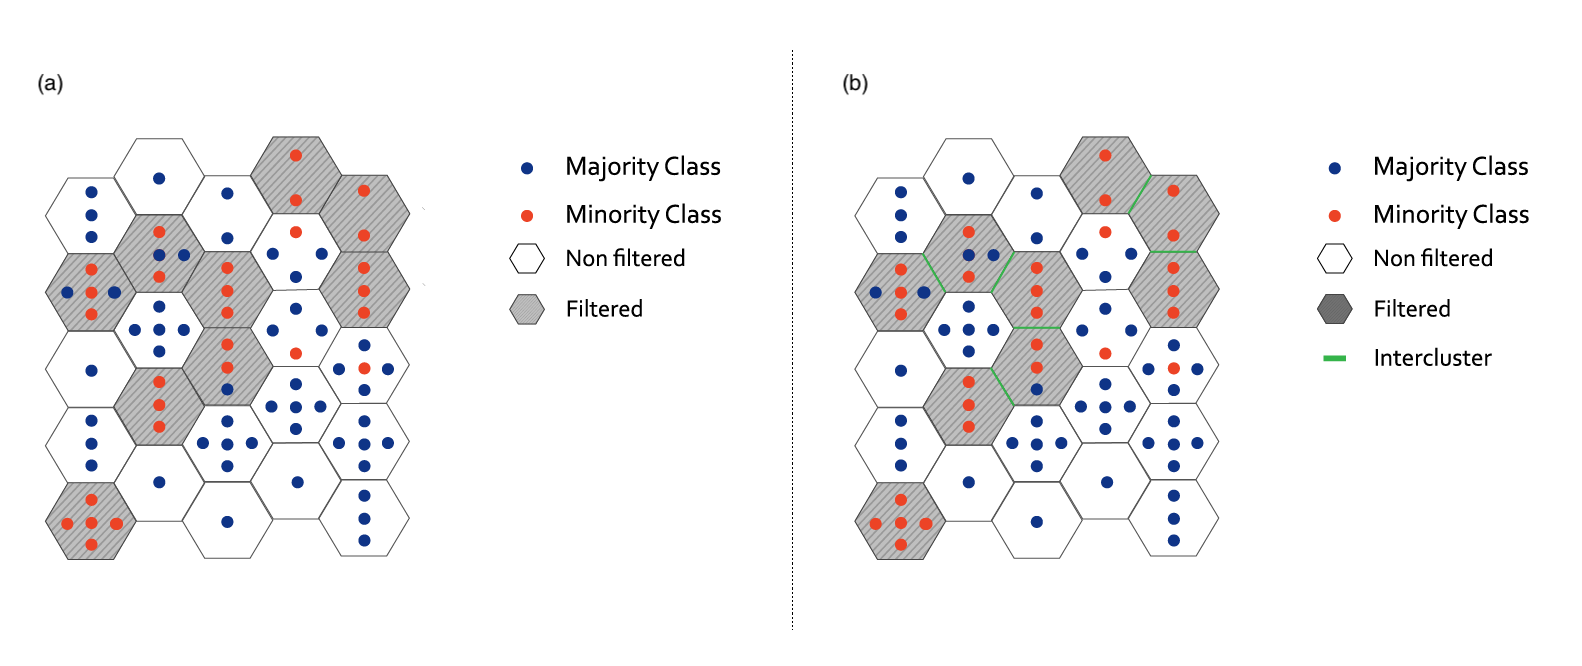
\includegraphics[width=18cm,height=13cm, keepaspectratio]{./resources/fig5.png}
	\captionbelow{Overview of identified filtered clusters and neighboring relations, adopted from \cite{Douzas2017}}
	\label{fig:Somo_Overview}
\end{figure}

\textbf{Step 7:} 

In previous steps, the numbers of required synthetic instances for each filtered
cluster and each neighboring pair of filtered clusters were calculated. The
following process, that corresponds to the G-SMOTE data generation mechanism, is
applied to each one of them individually. 

The set of minority instances is shuffled, minority instances are repetitively
selected, where each minority instance can be selected multiple times if the
number of required synthetic instances is higher than the number of minority
instances. The current selected minority sample of is named $x_{center}$. Based
on $x_{center}$ a selection strategy given by $a_{sel}$ is applied. The combined
selection strategy identifies $x_{surface}$, the final neighbor of $x_{center}$.
Both are used to define the geometric area where new instances are generated and
a radius $R$ is defined as their Euclidean distance. 

The data generation process starts by creating a unit hypersphere around the
origin, as it can be seen in figure \ref{fig:Hypersphere}a. This hypersphere is
going to be modified within the next steps. Initially, a random point
$e_{sphere}$ is created on the surface of the unit hypersphere. Subsequent,
$e_{sphere}$ is transformed to $x_{gen}$ a random point along the radius,
uniformly distributed. Next, a truncation is applied, a partition of the
hypersphere, as illustrated in \ref{fig:Hypersphere}b with $\alpha_{trunc}$
determining the degree of the truncation. Another transformation 5 deforms the
truncated hypersphere to a hyper spheroid, as it can be seen in
\ref{fig:Hypersphere}c The parameter $\alpha_{def}$ controls the degree of the
deformation.  As a final transformation we translate and rescale the point
$x_{gen}$ based on $x_{center}$ and the radius $R$.

\begin{figure}[H]
	\centering
	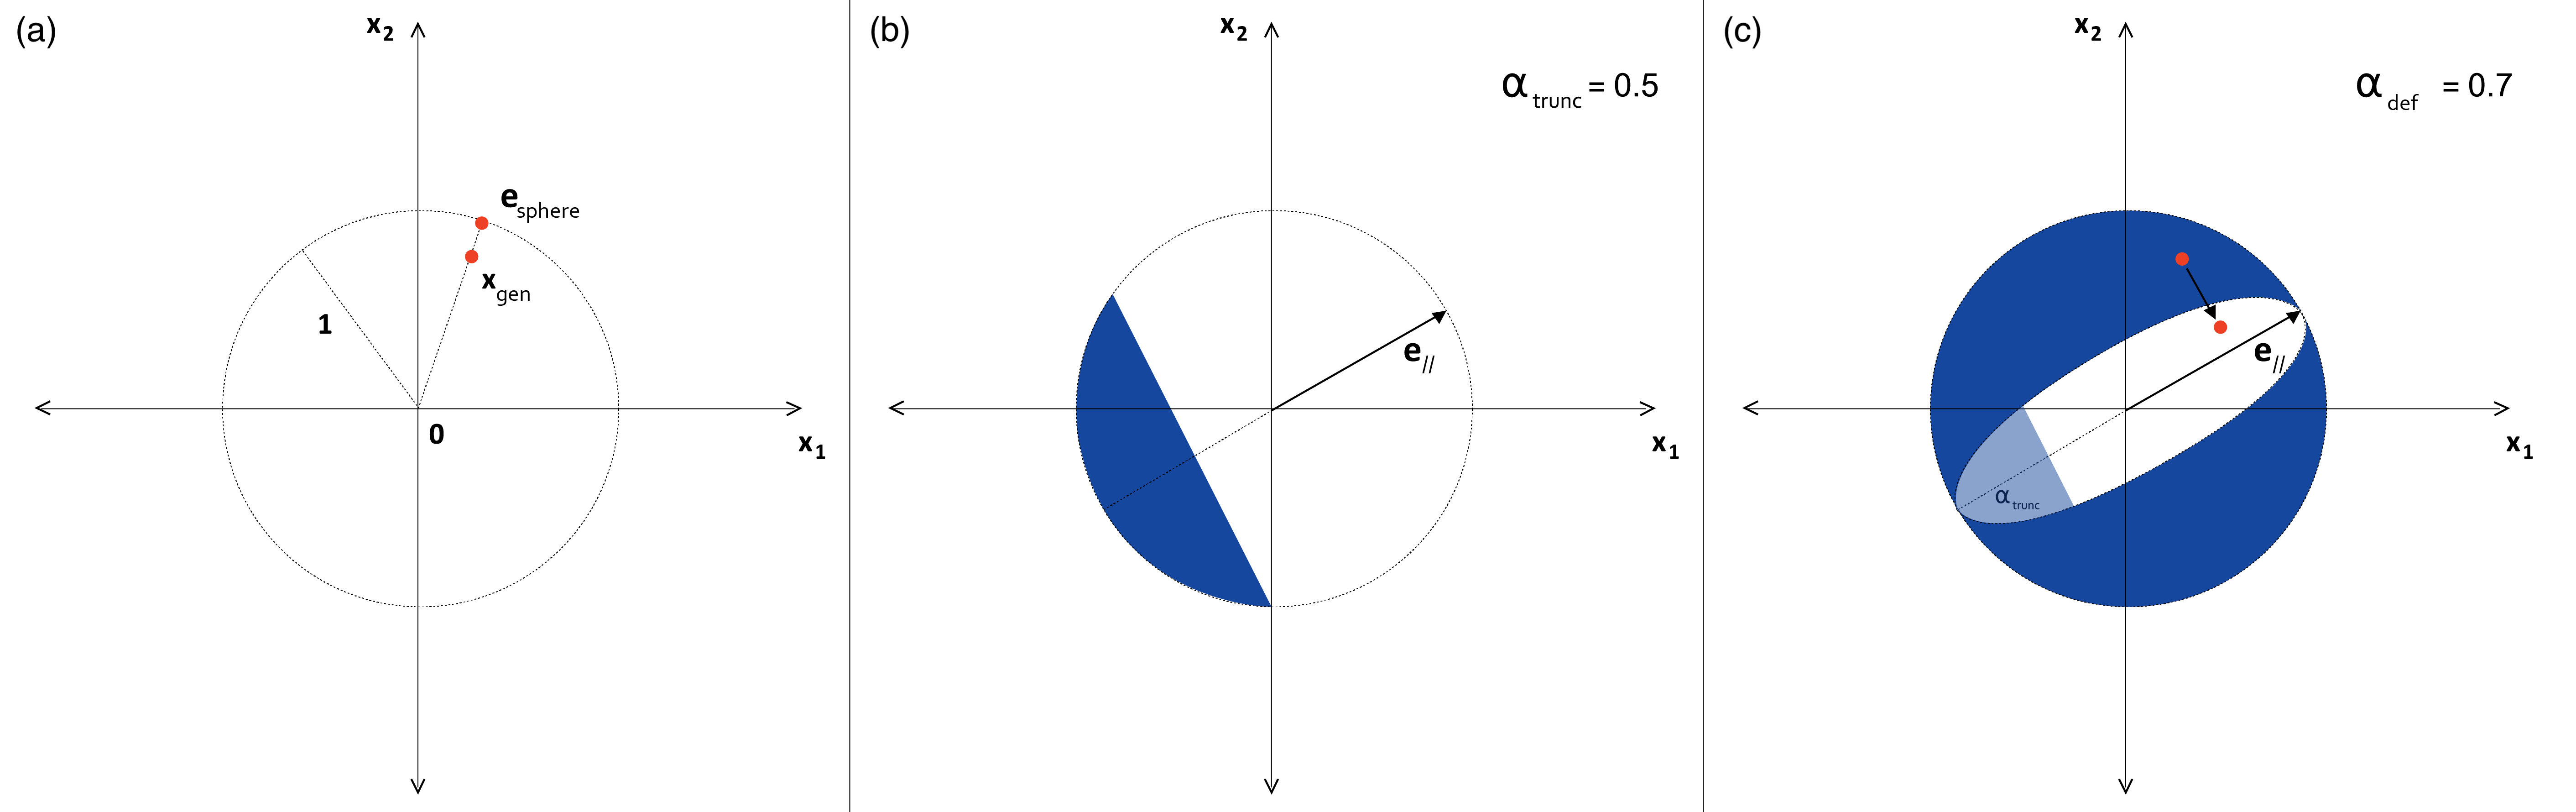
\includegraphics[width=15cm,height=10cm, keepaspectratio]{./resources/fig6.png}
	\captionbelow{Constructing the geometric region, based on the unit hyper sphere, truncation and 
	deformation, adopted from \cite{Douzas2017}}
	\label{fig:Hypersphere}
\end{figure}

The process is repeated until $N_{intra} + N_{inter}$ are generated. The final
output of the G-SOMO algorithm is the oversampled matrix $S'$, consisting of the
input data set and the set $S_{synthetic}$ of synthetic minority instances.

\section{Research methodology}

This section describes the evaluation process of G-SOMO using multiple
classifiers, datasets and metrics. The experimental data as well as the
experimental procedure is are presented in details, while a description of the
evaluation measures, the classification algorithms and the software
implementation is provided.

\subsection{Experimental data}

To ensure meaningful and significant insights we evaluated our models on a total
of 69 datasets. These datasets consist of commonly used datasets mainly from UCI
Machine Learning repository. In order to reach this high number of datasets, we
randomly undersampled the minority class of some of them to increase so that the
IR is increased. Using this approach, we managed to create additional and more
challenging datasets. Table 1 provides an overview of our datasets, the number
of features, instances and their IR:

\pgfplotstabletypeset[
begin table=\begin{longtable},
end table=\end{longtable},
col sep=comma,
header=true,
columns={Dataset name,Features,Instances,Minority instances,Majority instances,Imbalance Ratio},
columns/Dataset name/.style={column type=l,string type},
columns/Features/.style={fixed,fixed zerofill,precision=0,column type=r},
columns/Instances/.style={fixed,fixed zerofill,precision=0,column type=r},
columns/Minority instances/.style={fixed,fixed zerofill,precision=0,column type=r},
columns/Majority instances/.style={fixed,fixed zerofill,precision=0,column type=r},
columns/Imbalance Ratio/.style={fixed,fixed zerofill,precision=2,column type=r},
every head row/.style={before row=\toprule, after row=\midrule\endhead},
every last row/.style={after row=\bottomrule \caption{Overview of experimental data.}}
]
{./resources/datasets_summary.csv}

The data sets that can be download from  
\url{https://github.com/IMS-ML-Lab/publications/raw/master/assets/data/imbalanced_data.db}.

\subsection{Evaluation measures}

The model evaluation is based on different evaluation measures. Traditional
metrics, such as accuracy, show a strong bias towards the majority class and
should not be used on imbalanced datasets. The overall accuracy would seem to be
precise, even though the model might not perform well on the minority class. To
retrieve more accurate insights on the following evaluation measures are used: 

\begin{itemize}

	\renewcommand\labelitemi{--}

	\item Area Under The ROC Curve (AUC)
  
  	The ROC Curve is created by plotting the True Positive Rate against the
  	False Positive Rate as the decision threshold is changing \cite{Hand2009}.
	
	\item F-score
	  
	It is defined as the harmonic mean between precision and recall,
	assuming that both metrics are of equal importance \cite{Guo2018}
    
  	\item Geometric Mean Score (G-mean)
  
  	The geometric mean score, as the name implies, is defined as the geometric
  	mean between sensitivity and specificity.

\end{itemize}

\subsection{Machine learning algorithms} 

The goal of the paper is to validate the effectiveness of G-SOMO as an
oversampling method. Therefore G-SOMO was evaluated on the
aforementioned 69 datasets and compared to random
oversampling (RANDOM OVERSAMPLING) and SMOTE. Additionally, the performance of
the classifiers without applying any type of oversampling is also included in
the experimental results (NO OVERSAMPLING).

Different classifier algorithms are chosen to evaluate the performance of the
oversampling methods. It is crucial to ensure that the obtained results are
generalizable to different classifiers and not only to specific ones, due to the
different algorithms characteristics. The chosen classifiers are Logistic
Regression (LR) \cite{McCullagh1989}, K-Nearest Neighbors (KNN)
\cite{Cover1967}, Decision Tree (DT) \cite{Salzberg1994} and Gradient Boosting
Classifier (GBC) \cite{Friedman2001}.

\subsection{Experimental procedure}

In order to evaluate the performance of each combination of oversampler and
classifier, $n$-fold cross-validation was applied with $n = 5$. The data set was
split into $n$ different subsets (also called folds). $n-1$ folds were used to
train the classifier and generate artificial data by utilizing the oversampler
while the last fold remained unseen to validate. The process was applied in an
iterative manner, such that each fold was used for validation once. The
validation results of each model were averaged afterwards. The process was
repeated 3 times to avoid bias due to random grouping \cite{Japkowicz2013}.

A variety of hyper-parameters were used for the the oversamplers. For SMOTE the
optimal value of $k$ nearest neighbors was selected as $k \in \{3, 5 \}$. For
G-SOMO a hyper-parameter grid was generated from the Cartesian product of the
number of nearest neighbors $k \in \{3, 5\}$, the truncation factor 
$a_{trunc} \in \{−1.0, 0.0, 0.25, 1.0 \}$, the deformation factor $a_{def} \in \{0.0, 0.25, 1.0\}$, 
the dimension of the SOM grid $N_{Grid} \in \{20\%, 50\% \}$ in units
that correspond to the percentage of samples for each dataset and the ratio
$\frac{N_{intra}}{N_{intra} + N_{inter}} \in \{0.75, 1.0 \}$. The rest of G-SOMO
hyper-parameters are fixed to the following values: For each dataset $N_{intra} + N_{inter}$ 
is adjusted so that the oversampled dataset is perfectly balanced
while the selected strategy $\alpha_{sel}$ is the combined one. The threshold
$IR_{f}$ was set equal to $1.0$. 

Using the above hyper-parameters, the highest cross validation score for each
combination of datasets, classifiers, oversamplers and evaluation metrics was
reported. A ranking score was applied to compare the performance of the
oversampling methods, aggregated over all datasets. The ranking score for the
best performing method is 1, the worst performing methods is 4. The Friedman
test was applied to confirm the statistical significance of the ranking results
\cite{Guyon2003}. The Friedman test is used to detect differences for a set of
experimental attempts when normality assumption may not hold. In this case the
null hypothesis represents the situation in which the classifiers show an
identical performance, in terms of their mean ranking, independently of the
oversampling method and performance metric used. Additionally, the Holms test
was applied, using G-SOMO as the control method \cite{Guyon2003}. The Holms test
is a non-parametric version of the t-test, where the null hypothesis is whether
the proposed G-SOMO algorithm outperforms the other methods as the control
method.

\subsection{Software implementation}

The implementation of the classifiers and oversamplers are based on the Python
libraries Scikit-Learn \cite{Pedregosa2012} and Imbalanced-Learn
\cite{Lemaitre2016}. The function that prepares and runs any comparative
experiment can be found at
\url{https://github.com/georgedouzas/scikit-learn-extensions/blob/master/sklearnext/tools/imbalanced_analysis.py},
while the G-SOMO implementation is available at
\url{https://github.com/IMS-ML-Lab/scikit-learn-extensions/tree/master/sklearnext/over_sampling}.
Being fully integrated with the Scikit-Learn ecosystem they can be adjusted and
used for a variety of custom comparative studies. The experiments reported in
this paper as well as the analysis of their results are reproducible using the
scripts provided at \url{https://github.com/IMS-ML-Lab/publications}.

\section{Results and discussion}

\subsection{Comparative presentation}

In this section the performance of the different oversamplers is presented. The
results are analyzed, by applying various statistical tests, to establish their
significance. Additionally, a taxonomy of G-SMOTE hyper-parameters is presented
as well as guidelines for their tuning relative to the characteristics of the
imbalanced datasets.

\subsection{Comparative presentation}

The mean and standard error of cross validation scores across datasets for each combination of
classifiers, metrics and oversamplers are presented in Table 2:

\pgfplotstabletypeset[
begin table=\begin{longtable}, 
end table=\end{longtable},
col sep=comma, 
header=true, 
columns={Classifier,Metric,NO OVERSAMPLING,RANDOM OVERSAMPLING,SMOTE,G-SOMO}, 
columns/Classifier/.style={column type=l,string type}, 
columns/Metric/.style={column type=l,string type}, 
columns/NO OVERSAMPLING/.style={column type=l,string type}, 
columns/RANDOM OVERSAMPLING/.style={column type=l,string type}, 
columns/SMOTE/.style={column type=l,string type}, 
columns/G-SOMO/.style={column type=l,string type},
every head row/.style={before row=\toprule, after row=\midrule\endhead}, 
every last row/.style={after row=\bottomrule \caption{Results for mean cross validation scores of oversamplers across the datasets.}}
] 
{./resources/scores.csv}

Table 2 shows that G-SMOTE performs better on average than the
rest of the methods. Particularly, the mean and standard error of percentage
difference between G-SOMO and SMOTE is presented in Table 3:

\pgfplotstabletypeset[
begin table=\begin{longtable}, 
end table=\end{longtable},
col sep=comma, 
header=true, 
columns={Classifier,Metric,Difference},
columns/Classifier/.style={column type=l,string type},
columns/Metric/.style={column type=l,string type},
columns/Difference/.style={column type=l,string type}, 
every head row/.style={before row=\toprule, after row=\midrule\endhead}, 
every last row/.style={after row=\bottomrule \caption{Results for percentage difference between G-SOMO and SMOTE across the datasets.}}
]
{./resources/perc_diff_scores.csv}

For the purpose of a clear distinction between the oversampling methods, a
ranking score is introduced, ranging from 1 to 4. More precisely, 1 represents
the best performance, 4 the worst. Table 4 below illustrates the mean rank of
each oversampler on each metric and each classifier averaged across datasets: 

\pgfplotstabletypeset[
begin table=\begin{longtable},
end table=\end{longtable},
col sep=comma,
header=true,
columns={Classifier,Metric,NO OVERSAMPLING,RANDOM OVERSAMPLING,SMOTE,G-SOMO},
columns/Classifier/.style={column type=l,string type}, 
columns/Metric/.style={column type=l,string type}, 
columns/NO OVERSAMPLING/.style={column type=l,string type}, 
columns/RANDOM OVERSAMPLING/.style={column type=l,string type}, 
columns/SMOTE/.style={column type=l,string type}, 
columns/G-SOMO/.style={column type=l,string type},
every head row/.style={before row=\toprule, after row=\midrule\endhead},
every last row/.style={after row=\bottomrule \caption{Results for mean ranking of oversamplers across the datasets.}}
]
{./resources/ranking.csv} 

Based on the insights from the above tables we can conclude, that G-SOMO
successfully outperforms other oversampling methods, proven in combination with
various Metrics and Classifiers, averaged over all datasets. Figure
\ref{fig:MeanRanking} underlines the dominance of G-SOMO, the graph provides the
ranking results of each oversampler for any combination of classifier and
metric. We can see that throughout all experiments G-SOMO demonstrates the best
performance, significantly improving the results for all classifiers. Moreover,
it highlights the previously mentioned ranking between all oversampling methods.


\begin{figure}[H]
	\centering
	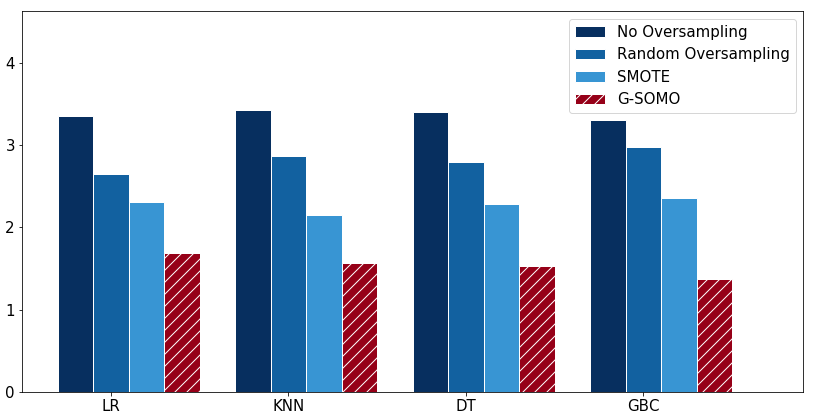
\includegraphics[width=15cm,height=12cm, keepaspectratio]{./resources/fig7.png}
	\captionbelow{Graphical overview of mean ranking for each classifier.}
	\label{fig:MeanRanking}
\end{figure}

\subsection{Statistical analysis} 

The results of the application of the Friedman test are shown in Table 5:

\pgfplotstabletypeset[
begin table=\begin{longtable},
	end table=\end{longtable},
col sep=comma,
header=true,
columns={Classifier,Metric,p-value,Significance},
columns/Classifier/.style={column type=l,string type},
columns/Metric/.style={column type=l,string type},
columns/p-value/.style={column type=r, zerofill, precision=1, dec sep align},
columns/Significance/.style={column type=r,string type},
every head row/.style={before row=\toprule, after row=\midrule\endhead},
every last row/.style={after row=\bottomrule \caption{Results for Friedman test.}}
]
{./resources/friedman_test.csv}

Therefore at a significance level of a = 0.05 the null hypothesis is rejected,
i.e. the classifiers do not perform similarly in the mean rankings across the
oversampling methods and evaluation metrics. Following the Friedman test, the
Holm's method is applied to adjust the p-values of the paired difference test
with G-SMOTE algorithm as the control method. The adjusted $\text{p-values}$ are
presented in Table 6:

\pgfplotstabletypeset[
begin table=\begin{longtable},
	end table=\end{longtable},
col sep=comma,
header=true,
columns={Classifier,Metric,NO OVERSAMPLING,RANDOM OVERSAMPLING,SMOTE},
columns/Classifier/.style={column type=l,string type},
columns/Metric/.style={column type=l,string type},
columns/NO OVERSAMPLING/.style={ zerofill,precision=1,column type=r, dec sep align},
columns/RANDOM OVERSAMPLING/.style={zerofill,precision=1,column type=r, dec sep align},
columns/SMOTE/.style={zerofill,precision=1,column type=r, dec sep align},
every head row/.style={before row=\toprule, after row=\midrule\endhead},
every last row/.style={after row=\bottomrule \caption{Adjusted p-values using the Holm's method.}}
]
{./resources/holms_test.csv}

Therefore, the null hypothesis of the Holm's test is rejected at a significance
level of a = 0.05 for 27 out of 36 total cases. It is important to note that the
search in the hyper-parameter space was very limited due to time and
computational restrictions, given that we used 69 datasets.

\subsection{Analysis and tuning of optimal hyper-parameters}

G-SOMO can be divided into two different categories. The first category is
related to the SOMO parametrization while the second category are the
$\alpha_{trunc}$, $\alpha_{def}$, $\alpha_{sel}$ hyper-parameters that control
the G-SMOTE data generation mechanism.

The most crucial hyper-parameter of the first category is the optimal size
$N_{Grid}$ of the SOM grid. After SOM training is applied, the high dimensional
input space will be transformed into a two-dimensional grid that consists of
$N_{Grid}^2$ clusters, which are used to identify safe areas for the data
generation process. The challenge hereby is to select a value allowing to
discriminate between sparse and dense minority class areas.  A very small value
will not be able to identify sub-clusters, since the identified clusters will
have a very large size of instances. Assuming a uniform distribution on the SOM
map, one can set the threshold to $\sqrt{|S_{min}|}$ to ensure that each cluster
contains on average one minority class. On the other hand, high values of
$N_{Grid}$ will result in smaller sized clusters, which might lead to filtered
clusters in areas that we would usually like to ignore, because they are
considered outliers. $\sqrt{|S_{maj}|}$ provides a reasonable upper bound for
$N_{Grid}$. The optimal value for $N_{Grid}$ is dependent on the characteristics
of the data set and can only be approximated in an experimental approach.

An analysis of the second category of G-SOMO hyper-parameters shows a dependence
on Imbalance Ratio (IR) as well as the number of samples over number of features
ratio (R). Specifically we can conclude the following: 

\begin{itemize}
	
	\renewcommand\labelitemi{--}

	\item High IR or low R.
	
	The \( majority \) (or \( combined \)) selection strategy and lower absolute
	values of the truncation and deformation factors dominate as optimal
	hyper-parameters.

	\item Low IR or high R. 
	
	The \( minority \) selection strategy and higher absolute values of the
	truncation and deformation factors dominate as optimal hyper-parameters.

\end{itemize}

\section{Conclusion}

In this paper, we proposed a new oversampling algorithm G-SOMO. The algorithm
observes the characteristics of the multidimensional data input while grouping
the input data to identify filtered clusters where minority instances dominate.
Within these filtered clusters, as well as between neighboring filtered
clusters, we create synthetic minority class instances. During their creation,
we apply the combined selection strategy, that also takes majority instances
into account. The synthetic instances are created in a safe hyper-spheroid.

G-SOMO was evaluated on 69 different datasets and compared to popular
oversampling methods. We validated the performance with different metrics, such
as the AUC, F-score and G-mean. In order to avoid dependence of the results to a
specific classifier, we chose multiple ones that differ in their
characteristics. Each experiment is repeated 3 times with a 5-fold
cross-validation. We proved the statistical significance of our results by
appropriate statistical tests.

In particular, our empirical results highlight the need for oversampling
algorithms. Utilizing no oversampling method produced the worst results in our
mean ranking, while simple methods like random oversampling increased the
performance when compared with it. The popular method SMOTE performed better
than the previous ones, whereas G-SOMO dominated the ranking and outperformed
other oversamplers.  Therefore, we are confident that G-SOMO is a new appealing
approach for researchers and practitioners working with imbalanced datasets. 

Future work will focus on a more efficient estimation of the algorithms
hyper-parameter. During our experiments we noticed the issue to be challenging,
through additional research one might identify generalizable characteristics for
the parameters based on the datasets characteristics. Additional improvements
can be expected through further research. Alternatively, the behavior of the
algorithm on imbalanced datasets with multiple target classes is worth to
explore, since research about oversampling on multi-class classification
problems is limited compared to the binary case. 

\bibliography{references}
\bibliographystyle{apalike}

\end{document}